Die  maximale Ausgangsleistung wurde grob berechnet  mit  $\SI{24}{\volt}  \cdot
\SI{3}{\ampere} = \SI{72}{\watt}$.

Da das Aufbauen eines eigenen Netzteils f\"ur die notwendige Ausgangsleistung zu
aufw\"andig und  teuer  gewesen  w\"are,  entschieden wir uns f\"ur ein externes
Netzger\"at  dass  im  Geh\"ause  montiert werden kann. Das verwendete  Netzteil
liefert   \SI{36}{\volt}   und   \SI{75}{\watt}  und  ist   in   der   Abbildung
\ref{fig:circuit:mains-input} als $N_2$ zu sehen.

\begin{figure}[th!]
    \center
    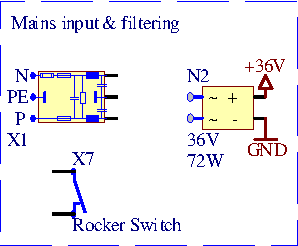
\includegraphics[width=.35\textwidth]{images/circuit/mains-input.pdf}
    \caption{Netzspannung wird gefiltert und auf 36V DC durch ein externes Netzmodul transformiert}
    \label{fig:circuit:mains-input}
\end{figure}

Weiter  wird  eine  Netzeingangs-Steckverbinder  mit integriertem Netzfilter und
Sicherung  verwendet,  was  in der Abbildung  \ref{fig:circuit:mains-input}  als
$X_1$  zu  sehen  ist. Ein auf der R\"uckseit des Geh\"auses montierter Schalter
$X_7$ erlaubt das Ein- und Ausschalten des Endproduktes.

